% Principal GDZ PPN236018647, native468–471upper; HKUST469–472.
\clearpage\SourceLeaf{468}\ArithmeticHead{461}{R}{GAUSS AN SCHUMACHER.}
\par\medskip\Needspace{4\baselineskip}\begin{center}[2]\end{center}
\begin{center}\textsc{Gauss} an \textsc{Schumacher}.\quad Göttingen, 21. März 1836.\end{center}
\HistoricCitation{[Briefwechsel zwischen \textsc{Gauss} und \textsc{Schumacher} III, Altona 1861, S. 13—14.]}
\indent .\enspace.\enspace.\enspace.\enspace.\enspace.\enspace.\quad Was Ihr Viereck betrifft, so heisst doch die Aufgabe so: Vier Pkte \(a,\ b,\ c,\ d\) sind gegeben, man soll einen 5\,ten \(x\) finden, so dass \(ax+bx+cx+dx\) ein Minimum wird, und das ist von den 3 Durchschnittspunkten \(ab\) mit \(cd\), \(ac\) mit \(bd\), \(ad\) mit \(bc\) der eine, wo man für die Auswahl die Bedingung entweder leicht auf Anschauung reduciren, oder analytisch einkleiden könnte. Lassen Sie nun \(a,\ b,\ c\) fest sein und \(d\) dem \(c\) immer näher rücken, so bleibt diese Auflösung noch immer so lange richtig, als Sie nicht \(c\) mit \(d\) zusammenfallen lassen. Fällt aber \(c\) mit \(d\) zusammen, so erfordert Geist und Buchstabe der \textls[120]{mathematischen} Aufgabe, als solcher, dass Sie dann \(c\) \textls[120]{zweimahl} zählen, also in dem Dreieck \(abc\) \(ax+bx+2cx\) zu einem Minimum machen, wo sich die allgemeine Auflösung noch immer als richtig ausweiset.

\indent Ist bei einem 4 Eck nicht von der stricten mathematischen Aufgabe, wie sie oben ausgesprochen ist, sondern von dem kürzesten Verbindungssystem die Rede, so werden mehrere einzelne Fälle von einander unterschieden werden müssen, und es bildet sich so eine recht interessante mathematische Aufgabe, die mir nicht fremd ist, vielmehr habe ich bei Gelegenheit einer Eisenbahnverbindung zwischen Harburg, Bremen, Hannover, Braunschweig sie in Erwägung genommen und bin selbst auf den Gedanken gekommen, dass sie eine ganz schickliche Preisfrage für unsre Studenten bei Gelegenheit abgeben könnte. Die Möglichkeit verschiedener Fälle erläutern wohl hinreichend folgende Figuren:
\begin{center}
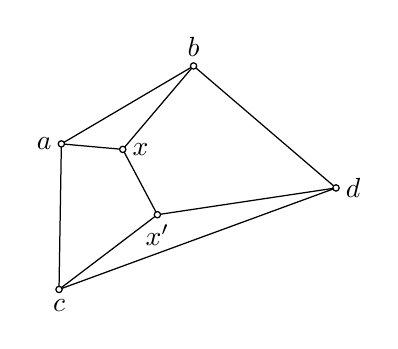
\begin{tikzpicture}[x=.010cm,y=-.010cm,line width=.45pt]
\draw (3,99)--(171,0)--(352,155)--(0,284)--cycle;
\draw (3,99)--(81,106)--(171,0);
\draw (81,106)--(125,189);
\draw (0,284)--(125,189)--(352,155);
\draw[fill=white] (3,99) circle[radius=4];
\draw[fill=white] (171,0) circle[radius=4];
\draw[fill=white] (352,155) circle[radius=4];
\draw[fill=white] (0,284) circle[radius=4];
\draw[fill=white] (81,106) circle[radius=4];
\draw[fill=white] (125,189) circle[radius=4];
\node[left] at (3,99) {$a$};
\node[above] at (171,0) {$b$};
\node[below] at (0,284) {$c$};
\node[right] at (352,155) {$d$};
\node[right] at (81,106) {$x$};
\node[below] at (125,189) {$x'$};
\end{tikzpicture}\hspace{.45cm}
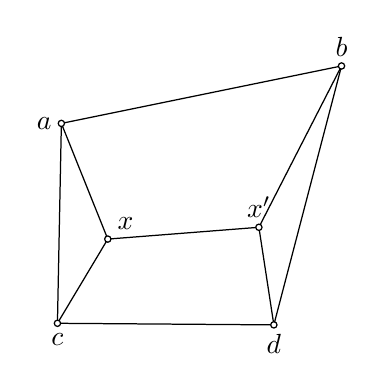
\begin{tikzpicture}[x=.010cm,y=-.010cm,line width=.45pt]
\draw (5,73)--(361,0)--(275,329)--(0,327)--cycle;
\draw (5,73)--(64,220)--(0,327);
\draw (64,220)--(256,205);
\draw (361,0)--(256,205)--(275,329);
\draw[fill=white] (5,73) circle[radius=4];
\draw[fill=white] (361,0) circle[radius=4];
\draw[fill=white] (0,327) circle[radius=4];
\draw[fill=white] (275,329) circle[radius=4];
\draw[fill=white] (64,220) circle[radius=4];
\draw[fill=white] (256,205) circle[radius=4];
\node[left] at (5,73) {$a$};
\node[above] at (361,0) {$b$};
\node[below] at (0,327) {$c$};
\node[below] at (275,329) {$d$};
\node[above right] at (64,220) {$x$};
\node[above] at (256,205) {$x'$};
\end{tikzpicture}\hspace{.45cm}
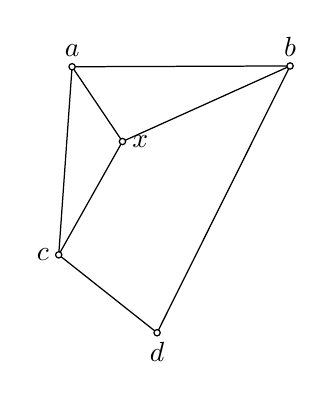
\begin{tikzpicture}[x=.010cm,y=-.010cm,line width=.45pt]
\draw (17,1)--(294,0)--(125,339)--(0,240)--cycle;
\draw (17,1)--(81,96)--(294,0);
\draw (81,96)--(0,240);
\draw[fill=white] (17,1) circle[radius=4];
\draw[fill=white] (294,0) circle[radius=4];
\draw[fill=white] (0,240) circle[radius=4];
\draw[fill=white] (125,339) circle[radius=4];
\draw[fill=white] (81,96) circle[radius=4];
\node[above] at (17,1) {$a$};
\node[above] at (294,0) {$b$};
\node[left] at (0,240) {$c$};
\node[below] at (125,339) {$d$};
\node[right] at (81,96) {$x$};
\end{tikzpicture}
\end{center}
\clearpage\SourceLeaf{469}\ArithmeticHead{462}{L}{GEOMETRIE. BRIEFWECHSEL.}
\noindent wo in der dritten Figur die Verbindung von \(c\) nach \(d\) direct gehen muss (was wirklich bei obigem Beispiel der Fall wird). Doch die Zeit drängt, also heute hiervon nicht mehr .\enspace.\enspace.\enspace.\enspace.\enspace.

\NumberedItem{3}
\begin{center}\textsc{Schumacher} an \textsc{Gauss}.\quad Altona, 2. April 1836.\end{center}
\HistoricCitation{[Briefwechsel zwischen \textsc{Gauss} und \textsc{Schumacher} III, Altona 1861, S. 24—25.]}
\indent \{.\enspace.\enspace.\enspace.\enspace.\enspace.\quad Bei Ihrem Problem der vortheilhaftesten Verbindung von 4 Städten, kann es auch vorkommen, dass eine Verbindung zwischen zweyen derselben ein grösseres Gewicht bekommt, weil diese Verbindung dem, der die Kosten der Eisenbahn hergiebt, wichtiger ist als die anderen. In diesem Falle würde die gebrochene Linie zwischen beiden Städten mehr der graden, die durch beide geht, genähert werden müssen. Ist es in dieser Rücksicht, dass die Verbindung von Braunschweig nach Hannover nach der graden Linie geht, also das höchste Gewicht hat, oder ist es von dem von mir erwähnten Gewicht abgesehen, eine Folge ihrer gegenseitigen Lage?\}

\NumberedItem{4}
\begin{center}\textsc{Schumacher} an \textsc{Gauss}.\quad Altona, 7. April 1836.\end{center}
\HistoricCitation{[Briefwechsel zwischen \textsc{Gauss} und \textsc{Schumacher} III, Altona 1861, S. 26—28.]}
\indent \{Ich muss Sie, mein theuerster Freund, noch einmal mit einer Kleinigkeit beschweren, nemlich mit der Auflösung der Aufgabe: wenn 4 Puncte gegeben sind, einen 5ten zu finden, von dem die an die gegebenen 4 gezogenen Linien ein Minimum sind. Ich kann nicht die in Ihrem Briefe angedeutete Auflösung, nemlich dass es einer von den Durchschnittspuncten der durch 2 dieser Puncte gezogenen Linien ist, finden. Um sie in den Stand zu setzen, besser darüber zu urtheilen, worin mein Fehler liegt, will ich Ihnen kurz darlegen, wie ich die Sache angegriffen habe.
\clearpage\SourceLeaf{470}\ArithmeticHead{463}{R}{SCHUMACHER AN GAUSS.}
\indent Zuerst nahm ich die Aufgabe sur le haut ton, und fing mit einer beliebigen Anzahl von Puncten an, deren rechtwinklichte Coordinaten \((a,b),\ (a',b'),\ (a'',b'')\ .\ .\ .\) u. s. w. sind. Wenn ich die Coordinaten des unbekannten Punctes \((x,y)\) setze, so ergeben sich gleich die Gleichungen
\[
\begin{aligned}
0&=\frac{x-a}{\surd\{(x-a)^2+(y-b)^2\}}+\frac{x-a'}{\surd\{(x-a')^2+(y-b')^2\}}\\
&\qquad{}+\frac{x-a''}{\surd\{(x-a'')^2+(y-b'')^2\}}+.\ .\ .\ \text{u. s. w.}\\[1em]
0&=\frac{y-b}{\surd\{(x-a)^2+(y-b)^2\}}+\frac{y-b'}{\surd\{(x-a')^2+(y-b')^2\}}\\
&\qquad{}+\frac{y-b''}{\surd\{(x-a'')^2+(y-b'')^2\}}+.\ .\ .\ \text{u. s. w.}
\end{aligned}
\]
\noindent Daraus fand ich dann, da \(\dfrac{y-b}{x-a}\) die Tangente des Winkels ist, den die durch die Puncte \((x,y),\ (a,b)\) gezogene Linie mit der Abscissenaxe\footnote{oder einer durch \((x,y)\) gezogenen Parallele mit der Abscissenaxe.} macht (diese Winkel mit \(w,\ w',\ w''\) u. s. w. bezeichnet), für das Minimum die beiden Gleichungen
\[
\text{(A)}\qquad\left\{\begin{aligned}
0&=\cos w+\cos w'+\cos w''+.\ .\ .\\
0&=\sin w+\sin w'+\sin w''+.\ .\ .,
\end{aligned}\right.
\]
\noindent und da die Lage der Abscissenaxe beliebig ist, da die gegebenen Abscissen, welche sich auf die angenommene Lage der Abscissenaxe bezogen, ganz aus diesen Ausdrücken verschwunden sind, so kann man die Winkel \(w,\ w',\ w''\ .\ .\ .\) von jeder beliebigen durch \((x,y)\) gezogenen Linie rechnen. Den Gleichungen (A) geschieht Genüge, wenn die vom \((x,y)\) an \((a,b),\ (a',b')\) u. s. w. gezogenen Linien lauter gleiche Winkel bilden, und für ein Viereck, dessen innere Winkel alle \(<180^{0}\) sind, durch den Durchschnittspunct der Diagonalen. Mehr kann ich aber nicht aus den Grundgleichungen herausbringen. Will ich \(x\) und \(y\) direct suchen, so komme ich auf mir unübersehbare Complication.

\indent Ich versuchte es noch für das Viereck auf eine andere Art. Sind \(A,\ B,\ C,\ D\) die gegebenen, \(X\) der gesuchte Punct, so nahm ich als Gegebene der Aufgabe \(a,\ b,\ c\) und die Winkel \(\alpha,\ \beta\), als Unbekannte die Winkel \(\varphi,\ u\). Die
\begin{center}
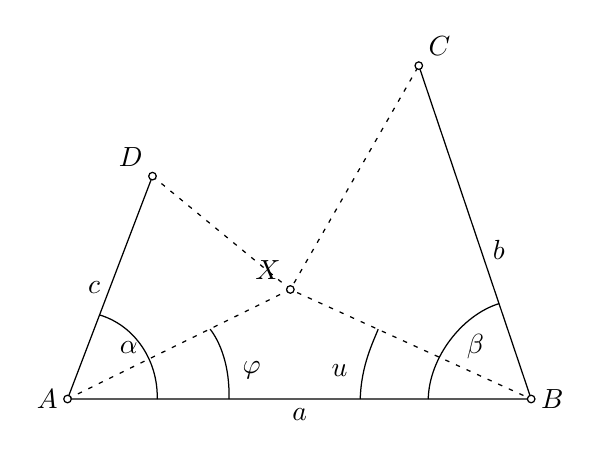
\begin{tikzpicture}[x=.012cm,y=-.012cm,line width=.45pt]
\draw (0,353)--(90,117);
\draw (0,353)--(491,353)--(372,0);
\draw[dash pattern=on 1.6pt off 2.6pt] (0,353)--(236,237)--(372,0);
\draw[dash pattern=on 1.6pt off 2.6pt] (90,117)--(236,237)--(491,353);
\draw (95,353) .. controls (96,312) and (71,275) .. (34,264);
\draw (171,353) .. controls (172,319) and (162,293) .. (151,279);
\draw (382,353) .. controls (383,309) and (418,264) .. (457,252);
\draw (310,353) .. controls (311,317) and (324,292) .. (329,279);
\draw[fill=white] (0,353) circle[radius=4];
\draw[fill=white] (491,353) circle[radius=4];
\draw[fill=white] (372,0) circle[radius=4];
\draw[fill=white] (90,117) circle[radius=4];
\draw[fill=white] (236,237) circle[radius=4];
\node[left] at (0,353) {$A$};
\node[right] at (491,353) {$B$};
\node[above right] at (372,0) {$C$};
\node[above left] at (90,117) {$D$};
\node[above left] at (236,237) {$X$};
\node[below] at (246,353) {$a$};
\node[right] at (440,195) {$b$};
\node[left] at (45,235) {$c$};
\node at (65,299) {$\alpha$};
\node at (432,298) {$\beta$};
\node[right] at (175,323) {$\varphi$};
\node[left] at (307,323) {$u$};
\end{tikzpicture}
\end{center}
\clearpage\SourceLeaf{471}\ArithmeticHead{464}{L}{GEOMETRIE. BRIEFWECHSEL.}
\noindent Function
\[
\begin{aligned}
U={}&a\frac{\sin u}{\sin(\varphi+u)}+a\frac{\sin\varphi}{\sin(\varphi+u)}
+\surd\!\left(\frac{aa\sin\varphi^2}{\sin(\varphi+u)^2}+bb-2ba\frac{\sin\varphi}{\sin(\varphi+u)}\cos(\beta-u)\right)\\[1em]
&+\surd\!\left(\frac{aa\sin u^2}{\sin(\varphi+u)^2}+cc-2ca\frac{\sin u}{\sin(\varphi+u)}\cos(\alpha-\varphi)\right)
\end{aligned}
\]
\noindent soll dann ein Minimum seyn. Die Gleichungen \(\dfrac{\partial U}{\partial\varphi}=0\) und \(\dfrac{\partial U}{\partial u}=0\) sind aber auch für mich zu complicirt.

\indent Möchten Sie wohl, mein theuerster Freund, wenn Sie einen freien Augenblick haben, mir Ihre Methode mittheilen? Man könnte es wohl, wenn man sich gleiche Gewichte an 4 von einem Punct ausgehenden Fäden hängend vorstellte, die über Rollen in den Puncten \(A,\ B,\ C,\ D\) gingen, machen; wo dann das Gleichgewicht zu suchen wäre, bei dem die Gewichte den Verbindungspunct der Fäden in den gesuchten ziehen würden. Will man dann einigen Puncten eine grössere verhältnissmässige Wichtigkeit beilegen, so lässt sich das leicht durch grösseres an diesen Puncten angebrachtes Gewicht ausdrücken. Ich vermuthe aber, Sie haben einen rein analytischen oder geometrischen Weg gewählt .\enspace.\enspace.\enspace.\enspace.\}
